\documentclass[11pt]{article}

% ===================================================================
% EMNLP submission. For the official submission, this file expects the
% ACL style files (acl.sty, acl_natbib.bst) in the project root --
% available from the ACL ARR template gallery on Overleaf.
% Compile: pdfLaTeX -> pdfLaTeX (bibliography is inline; no BibTeX run needed).
% ===================================================================
\usepackage[review]{acl}

\usepackage{times}
\usepackage{latexsym}
\usepackage[T1]{fontenc}
\usepackage[utf8]{inputenc}
\usepackage{microtype}
\IfFileExists{inconsolata.sty}{\usepackage{inconsolata}}{}
\usepackage{graphicx}
\usepackage{booktabs}
\usepackage{amsmath}
\usepackage{multirow}

\graphicspath{{figures/}{./}}

\title{Diagnosing Probing Claims About Future Tokens with\\
Position Baselines and Training Dynamics}

\author{Anonymous Authors \\
  Anonymous Affiliation \\
  \texttt{anonymous@email} \\}

\begin{document}
\maketitle

\begin{abstract}
When a linear probe recovers information about a \emph{future} token from a
language model's hidden state, it is tempting to read this as evidence that the
model is \emph{planning} ahead. We show that such probe accuracies are
\emph{baseline-dependent} and conflate two distinct sources: positional
structure already present at initialization, and computation the model
\emph{learns} during training. We introduce a per-position \emph{staircase}
baseline that compares a target-position probe against the strongest earlier
position, and a \emph{training-dynamics decomposition} that splits the
resulting gap into a positional \emph{floor} (measured at random initialization)
and a \emph{learned} component (acquired during training). Applying this
diagnostic to 19 models across nine architecture families and five tasks
(116 probing experiments), we find that a \emph{single} methodology produces
three qualitatively different signatures: a large learned component for rhyme
(genuine forward planning, consistent with prior causal steering results),
a flat positional floor for code return-types (an artifact that vanishes under
a mean-pool baseline), and an absent signal for a controlled question-answering
task. The decomposition is consistent across three model scales
(1.4B--6.9B), and a within-model checkpoint analysis shows that the rhyme probe
gap and behavioral rhyme generation emerge together during training
(Spearman $\rho=0.75$, $p=0.03$). Our results argue that probing claims about
planning should be evaluated against position baselines and training dynamics
rather than raw probe accuracy.
\end{abstract}

\section{Introduction}
\label{sec:intro}

Linear probes are a standard tool for asking what information a language
model's hidden states contain \citep{alain2017,belinkov2022}. A recent and
striking application probes for information about \emph{future} tokens: if a
hidden state at position $t$ already encodes a property of a token that the
model has not yet generated, this is read as evidence that the model is
\emph{planning} ahead rather than predicting one token at a time. Causal
steering work supports this interpretation in some settings: \citet{maar2026}
show that steering vectors applied at intermediate positions can manipulate
future rhymes and question answers in models from 1B parameters upward.

Probing alone, however, is a fragile basis for planning claims. Probing
classifiers can exploit confounds and recover information that is not
\emph{used} by the model \citep{hewitt2019,belinkov2022}, and the distinction
matters precisely because probing is far cheaper to scale than causal
intervention---making it tempting to treat probe accuracy as a proxy for
mechanistic evidence. The central question of this paper is methodological:
\emph{when a probe recovers future-token information, how much of that signal
reflects model computation, versus information already recoverable from earlier
token positions?}

We argue that a raw probe accuracy answers this question only relative to a
baseline, and that the natural baselines have been too weak. We make three
contributions.

\textbf{(1) A per-position staircase baseline.} For each task we compare the
target-position probe against the \emph{single strongest earlier position}
(Section~\ref{sec:staircase}). This is a stricter baseline than the mean-pooled
``signature region'' baseline used in prior work, and it already changes the
picture: tasks that look like planning under weak baselines often do not survive
a per-position comparison.

\textbf{(2) A training-dynamics decomposition.} Probing a model at random
initialization isolates the part of any staircase gap that is purely
\emph{positional}---it requires no learning. Subtracting this \emph{floor} from
the trained model's gap yields the \emph{learned} component
(Section~\ref{sec:decomp}). This decomposition is, to our knowledge, a novel way
to separate positional artifacts from acquired computation in future-token
probing.

\textbf{(3) A large-scale, multi-architecture evaluation.} We apply the
diagnostic to 19 models spanning nine architecture families, five tasks, and
(for three Pythia scales) eight training checkpoints---116 probing experiments
in total, with linear and MLP probes, two baselines, and behavioral validation.

The result is not a single ``planning'' verdict but a \emph{discriminating
diagnostic}. The same methodology yields three qualitatively different
signatures (Figure~\ref{fig:dynamics}): rhyme couplets show a large gap that
\emph{grows} during training and persists under every baseline (genuine forward
planning); code return-type prediction shows a small gap that is \emph{flat}
across training and \emph{collapses} under a mean-pool baseline (a positional
artifact); and a controlled neutral-QA task shows \emph{no} gap at any training
stage (a genuine null). We further show, within a single model across training,
that the rhyme probe gap and the model's behavioral rhyme-generation ability
emerge together. The takeaway for practitioners is concrete: future-token
probing claims should be reported relative to a per-position baseline and,
where checkpoints are available, decomposed against the positional floor.

\section{Related Work}
\label{sec:related}

\paragraph{Probing and its confounds.} Linear probing
\citep{alain2017,conneau2018} is widely used to test what representations
encode, but \citet{hewitt2019} showed that probe accuracy conflates information
in the representation with the probe's own capacity, motivating control tasks
and selectivity. \citet{belinkov2022} surveys these limitations. Our staircase
is in this tradition: it replaces an absolute accuracy with a difference against
a position-matched baseline, and the training-dynamics floor plays a role
analogous to a control task but derived from the model itself.

\paragraph{Future-token information and planning.} A growing literature asks
whether language models represent future tokens. Future Lens \citep{pal2023}
decodes future tokens from individual hidden states; \citet{maar2026} provide
causal steering evidence for implicit planning in rhyme and question answering.
Our work is complementary and deliberately diagnostic: rather than adding
another planning claim, we ask how much of a probing signal would survive a
stricter baseline and how much is acquired during training.

\paragraph{Interpreting hidden states across layers and training.} The logit
lens \citep{nostalgebraist2020} and tuned lens \citep{belrose2023} read hidden
states through the unembedding; the Pythia suite \citep{biderman2023} enables
analysis across training checkpoints. We use checkpoints not to track loss but
to define a positional floor and to correlate representational change with
behavioral change.

\section{Method}
\label{sec:method}

\subsection{The per-position staircase}
\label{sec:staircase}

Each task provides prompts $x$ with a categorical label $y$ describing a
\emph{future} token (e.g.\ the rhyme family of an upcoming line-ending word).
For a model with hidden states $h^{(\ell)}_p(x)$ at layer $\ell$ and position
$p$, and a designated \emph{target} position $t(x)$ (e.g.\ the newline before
the upcoming line), we train probes at the target and at every earlier position.
Writing $\mathrm{acc}^{(\ell)}_p$ for the cross-validated accuracy of a probe
trained on activations at layer $\ell$, position $p$, the \emph{staircase gap}
at layer $\ell$ is
\begin{equation}
\label{eq:gap}
\Delta^{(\ell)} \;=\; \mathrm{acc}^{(\ell)}_{t}
\;-\; \max_{p < t}\, \mathrm{acc}^{(\ell)}_{p}.
\end{equation}
The baseline is the \emph{single strongest} earlier position, not an average:
if any earlier position already carries the label, $\Delta$ is small or
negative. We report the \emph{headline gap} as the largest-magnitude
$\Delta^{(\ell)}$ across probed layers and target-position resolvers, together
with a 500-sample bootstrap confidence interval. A positive gap is necessary
(not sufficient) evidence that the target position adds future-token information
beyond what is already linearly recoverable earlier.

\subsection{Dual baselines}
\label{sec:dual}

The max-earlier baseline of Eq.~\ref{eq:gap} is strict, but it compares single
positions. As a second, independent baseline we also probe the
\emph{mean-pooled} activations over all positions up to the signature region
(the ``$N{+}P$'' baseline of prior work), giving a gap
$\Delta_{\text{mp}}$. A signal that reflects genuine target-position
computation should survive both baselines; a positional artifact may survive the
single-position comparison yet collapse against a pooled representation that
aggregates the same information from many earlier tokens.

\subsection{Training-dynamics decomposition}
\label{sec:decomp}

A staircase gap at a \emph{trained} model mixes two things: structure that is
present before any learning (token identity in the embedding, positional
encoding) and computation acquired during training. We separate them using
checkpoints. Let $\Delta_{0}$ be the headline gap measured at
random initialization (step 0) and $\Delta_{\text{final}}$ the gap at the end of
training. We define
\begin{align}
\text{floor} &= \Delta_{0}, \\
\text{learned} &= \Delta_{\text{final}} - \Delta_{0}.
\end{align}
The floor is the gap attributable purely to position and embedding; the learned
component is what training adds. A large learned component is the signature we
associate with acquired forward planning; a near-zero learned component
(regardless of the raw gap) indicates a positional artifact. We test
significance of the learned component with a permutation test over examples.

\subsection{Probing setup}
\label{sec:probing}

Probes are logistic-regression classifiers on PCA-reduced activations
(128 components by default) with stratified cross-validation. For the
neutral-QA task, where prompts are grouped into minimal pairs that share
surface text, we use \emph{grouped} cross-validation (\texttt{StratifiedGroupKFold})
and cluster bootstrap so that paired prompts never straddle the train/test split;
this corrects an optimistic bias that ungrouped splitting introduces
(Appendix~\ref{app:grouped}). We additionally fit two-layer MLP probes to test
whether findings are artifacts of probe linearity (Section~\ref{sec:mlp}). We
report a bag-of-words baseline per task to flag cases where the label is
trivially recoverable from surface tokens.

\section{Experimental Setup}
\label{sec:setup}

\subsection{Tasks}
\label{sec:tasks}

We study five tasks chosen to span the space from genuine forward planning to
trivial surface prediction (Table~\ref{tab:tasks}). \textbf{Rhyme} uses the
couplet data of \citet{maar2026}: the model must commit to a rhyme family before
generating the rhyming word, and steering at the target positions causally
changes the produced rhyme. \textbf{Code} is return-type prediction over Python
functions; the function signature carries return-type cues, so the target
position is not expected to add information. \textbf{QA-neutral} uses minimal
question pairs that share \emph{identical} surface text across answers, so the
label cannot be read off earlier tokens; it is our cleanest test for planning in
the absence of surface confounds. \textbf{QA-suggestive} uses questions whose
surface content predicts the answer (a weak-gap control), and \textbf{Trivia}
uses questions whose content fully determines the answer category (a
bag-of-words--saturating null).

\begin{table}[t]
\centering\small
\begin{tabular}{@{}lccp{3.4cm}@{}}
\toprule
\textbf{Task} & \textbf{Cls.} & \textbf{$N$} & \textbf{Expected signal} \\
\midrule
Rhyme & 10 & 200 & Forward planning \\
QA-neutral & 2 & 161 & Planning, no surface cue \\
Code & 5 & 507 & Local / positional \\
QA-suggestive & 2 & 145 & Weak (surface cue) \\
Trivia & 5 & 100 & None (BoW-saturated) \\
\bottomrule
\end{tabular}
\caption{The five tasks, number of label classes, examples, and the
\emph{a priori} expectation for the staircase signal.}
\label{tab:tasks}
\end{table}

\subsection{Models}
\label{sec:models}

We evaluate 19 models spanning nine architecture families: Gemma-2
(2B/2B-it/9B/27B), Qwen3 (1.7B/8B), Pythia (410M--6.9B), GPT-2
(small/medium/XL), Mistral-7B, Llama-3.1-8B, Llama-3.2-3B, Falcon3-7B, OLMo-7B,
and StableLM-2-1.6B. These cover absolute, rotary, and RoPE-with-normalization
positional schemes. For the training-dynamics decomposition we use the three
deduplicated Pythia scales (1.4B, 2.8B, 6.9B) for which intermediate checkpoints
are released \citep{biderman2023}, probing at steps
$\{0, 512, 4\mathrm{k}, 16\mathrm{k}, 32\mathrm{k}, 64\mathrm{k},
128\mathrm{k}, 143\mathrm{k}\}$.

\section{Results}
\label{sec:results}

\subsection{The staircase gap is baseline-dependent and varies by an order of
magnitude across tasks}
\label{sec:res-cross}

\begin{figure}[t]
\centering
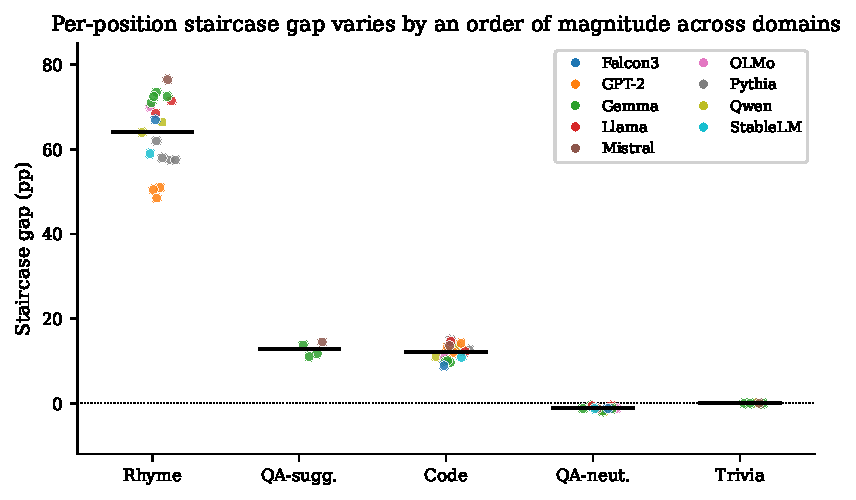
\includegraphics[width=\columnwidth]{fig2_cross_model.pdf}
\caption{Per-position staircase gap by task, one point per model, colored by
architecture family; black bars are task means. The gap separates rhyme
(+64pp mean) from code and QA-suggestive ($\sim$+12pp), QA-neutral
($\sim$0), and trivia (0). The ordering is consistent across all nine
architecture families.}
\label{fig:cross}
\end{figure}

Figure~\ref{fig:cross} shows the headline gap for every (model, task) pair.
The gap varies by an order of magnitude across tasks and is remarkably
consistent within a task across architectures. Rhyme yields a large positive
gap on all 19 models (mean $+63.6$pp, range $[+48.5, +76.5]$); code and
QA-suggestive yield small positive gaps (means $+12.0$ and $+12.7$pp);
QA-neutral yields a small \emph{negative} gap (mean $-1.2$pp, range
$[-1.9,-0.6]$); and trivia yields exactly zero, because its label is already
saturated by a bag-of-words baseline. A paired Wilcoxon test across models
confirms rhyme exceeds code (median difference $+53$pp, $n{=}18$,
$p<10^{-4}$) and QA-neutral (median $+72$pp, $n{=}12$, $p<10^{-3}$).

That rhyme stands apart is expected; the methodological point is that
the \emph{same} measurement, applied uniformly, places three tasks
(code, QA-suggestive, QA-neutral) near or below the floor despite their being
the kind of future-token tasks for which raw probe accuracy is high. A positive
probe accuracy is not a positive gap.

\subsection{Training dynamics decompose the gap into a positional floor and a
learned component}
\label{sec:res-dynamics}

\begin{figure}[t]
\centering
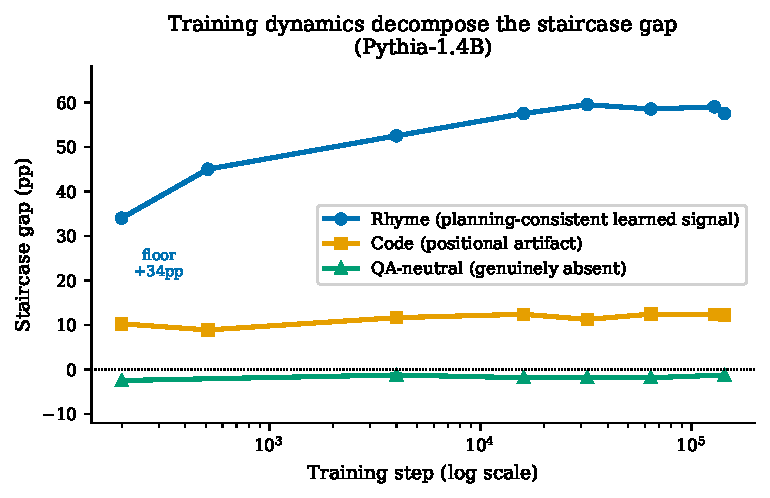
\includegraphics[width=\columnwidth]{fig1_training_dynamics.pdf}
\caption{Staircase gap across training (Pythia-1.4B, log-scale steps). Rhyme
(blue) starts at a $+34$pp floor and \emph{grows} to $+58$pp; code (orange)
is \emph{flat} near $+11$pp throughout; QA-neutral (green) sits at zero at every
checkpoint. A single methodology yields three qualitatively different
trajectories.}
\label{fig:dynamics}
\end{figure}

Probing across training checkpoints reveals \emph{why} the tasks differ
(Figure~\ref{fig:dynamics}). At random initialization, rhyme already shows a
$+34$pp gap---a substantial positional floor, since rhyme labels correlate with
token identity that the embedding exposes. But the gap then \emph{grows} to
$+58$pp over training: training adds $+23.5$pp of learned computation. Code, by
contrast, starts at a $+10$pp floor and stays flat (learned $+2$pp): training
adds essentially nothing at the target position. QA-neutral sits at zero at
every checkpoint, including step 0: the target position never carries the label,
trained or not.

A permutation test on the learned component is significant for both
rhyme and code on Pythia-1.4B and 2.8B ($p<10^{-3}$ for rhyme;
$p<10^{-3}$ and $p{=}9\times10^{-4}$ for code), but the \emph{magnitudes} tell
the story: a $+2$--$4$pp learned gap for code versus $+19$--$26$pp for rhyme.
The decomposition, not the raw significance, is what distinguishes acquired
computation from a stable positional artifact.

\subsection{The decomposition is consistent across model scale}
\label{sec:res-scale}

\begin{figure}[t]
\centering
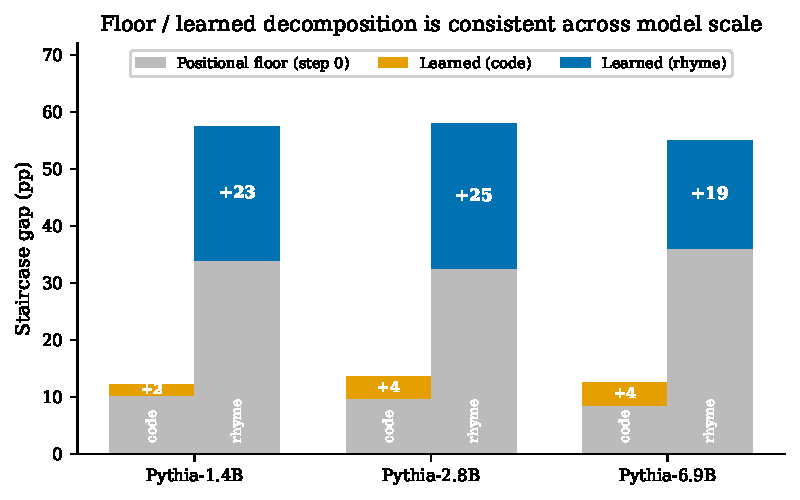
\includegraphics[width=\columnwidth]{fig3_decomposition.pdf}
\caption{Floor/learned decomposition for code and rhyme at three Pythia scales.
The positional floor (grey) and learned component (color) are stable across an
order of magnitude in parameters: code learns $+2$--$4$pp, rhyme learns
$+19$--$26$pp.}
\label{fig:decomp}
\end{figure}

Table~\ref{tab:decomp} and Figure~\ref{fig:decomp} repeat the decomposition on
Pythia-1.4B, 2.8B, and 6.9B. The pattern is stable across an order of magnitude
in scale: the code floor is $+8$--$10$pp with a $+2$--$4$pp learned component,
while the rhyme floor is $+33$--$36$pp with a $+19$--$26$pp learned component.
The consistency across three independently trained models indicates the
decomposition reflects a property of the task--representation interaction, not
an idiosyncrasy of one model.

\begin{table}[t]
\centering\small
\begin{tabular}{@{}lcccccc@{}}
\toprule
& \multicolumn{3}{c}{\textbf{Code}} & \multicolumn{3}{c}{\textbf{Rhyme}} \\
\cmidrule(lr){2-4}\cmidrule(lr){5-7}
\textbf{Model} & flr & fin & lrn & flr & fin & lrn \\
\midrule
Pythia-1.4B & 10.3 & 12.2 & 2.0 & 34.0 & 57.5 & 23.5 \\
Pythia-2.8B & \phantom{0}9.7 & 13.6 & 4.0 & 32.5 & 58.0 & 25.5 \\
Pythia-6.9B & \phantom{0}8.5 & 12.6 & 4.1 & 36.0 & 55.0 & 19.0 \\
\bottomrule
\end{tabular}
\caption{Floor / final / learned staircase gap (pp) for code and rhyme across
three Pythia scales. Code's learned component is near zero at every scale;
rhyme's is an order of magnitude larger.}
\label{tab:decomp}
\end{table}

\subsection{A mean-pool baseline confirms the code gap is positional}
\label{sec:res-dual}

\begin{figure}[t]
\centering
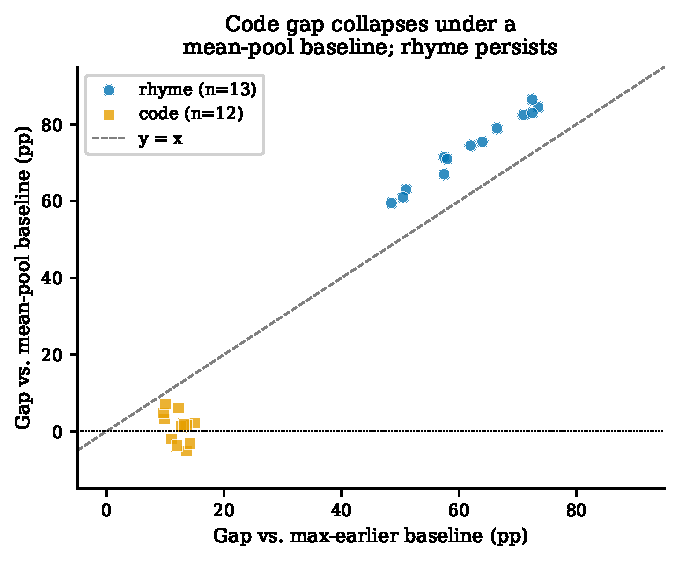
\includegraphics[width=0.85\columnwidth]{fig4_dual_baseline.pdf}
\caption{Each point is a model: staircase gap under the max-earlier baseline
($x$) versus the mean-pool baseline ($y$). Rhyme (blue) lies near the diagonal,
persisting under both baselines ($+59$ to $+86$pp). Code (orange) collapses to
the $x$-axis ($-5$ to $+7$pp): its single-position gap disappears once earlier
positions are pooled.}
\label{fig:dual}
\end{figure}

The training-dynamics view is corroborated by the second baseline
(Figure~\ref{fig:dual}). Under the mean-pool baseline, the code gap collapses to
$[-5.1, +7.1]$pp across models---i.e.\ pooling earlier positions recovers as much
return-type information as the target position---while the rhyme gap remains
large ($[+59.5, +86.5]$pp). Two independent baselines (a stricter single-position
comparison through training, and a pooled comparison) thus agree: the code
signal is recoverable from earlier positions, and the rhyme signal is not.

\subsection{Behavioral validation: the rhyme gap and rhyme generation emerge
together}
\label{sec:res-behav}

\begin{figure}[t]
\centering
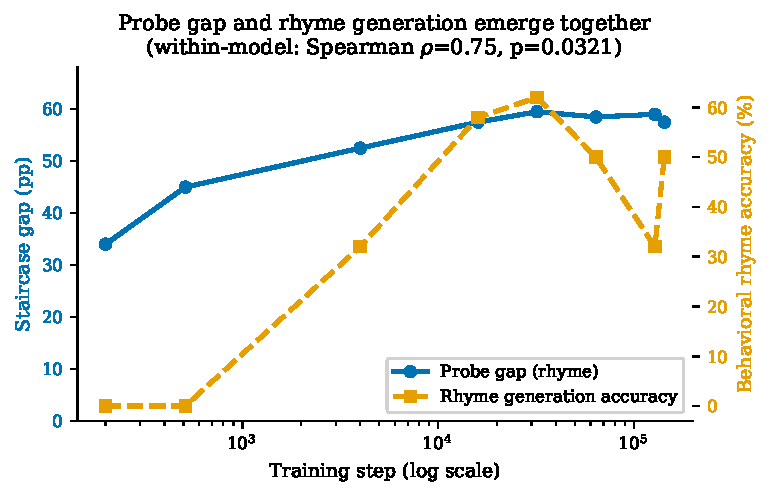
\includegraphics[width=\columnwidth]{fig5_behavioral.pdf}
\caption{Within-model behavioral validation (Pythia-1.4B). As training proceeds,
the rhyme staircase gap (blue) and the model's actual rhyme-generation accuracy
(orange) rise together; both emerge between steps 4k--32k. Within-model
Spearman $\rho=0.75$ ($p=0.03$); Pearson $r=0.88$ ($p=0.004$), $n=8$
checkpoints.}
\label{fig:behav}
\end{figure}

If the rhyme gap reflects acquired planning, it should track the model's actual
ability to produce rhymes. We measure behavioral rhyme-generation accuracy
(does the model complete a couplet with a correctly rhyming word, scored with a
pronunciation dictionary) at each Pythia-1.4B checkpoint and compare it to the
probe gap (Figure~\ref{fig:behav}). The two emerge together: at initialization
both are at floor (0\% generation, $+34$pp probe), and both rise sharply between
steps 4k and 32k. The within-model correlation is strong
(Spearman $\rho=0.75$, $p=0.03$; Pearson $r=0.88$, $p=0.004$; $n=8$).

We note an important negative result. The \emph{cross-model} correlation between
probe gap and generation accuracy is \emph{not} significant
($\rho=0.17$, $p=0.52$, $n=17$): a larger probe gap in model $A$ than model $B$
does not imply $A$ generates better rhymes. This is expected---generation
quality depends on decoding, tokenization, and scale, not only on whether the
information is linearly present---and it is why the within-model, across-training
comparison (which holds architecture and tokenizer fixed) is the appropriate
test. We report both to avoid overclaiming: the probe gap measures
\emph{representation}, which is necessary but not sufficient for behavior.

\subsection{Robustness: MLP probes and architecture coverage}
\label{sec:mlp}

The findings are not artifacts of linear probing. We refit the rhyme and
QA-neutral staircases with two-layer MLP probes on six models across four
families; in all 13 runs the MLP agrees with the linear probe in sign and
regime (large positive for rhyme, near-zero for QA-neutral;
Appendix~\ref{app:mlp}, Figure~\ref{fig:mlp}). Architecture coverage is broad:
the rhyme gap is $+48$ to $+77$pp on all nine families and is size-invariant
from 0.12B to 27B parameters (Appendix~\ref{app:size},
Figure~\ref{fig:size}). A floor analysis grouping models by positional-encoding
scheme finds the rhyme floor's positional component is essentially identical
across rotary, RoPE, and absolute schemes, indicating it is not an artifact of
one positional encoding.

\section{Discussion}
\label{sec:discussion}

\paragraph{What the staircase does and does not show.} The staircase is a
diagnostic for \emph{evidential strength}, not a claim that a capability is
absent. A near-zero or negative gap means the probe has not demonstrated
target-position information beyond what earlier positions already provide; it
does not prove the model lacks the relevant computation, nor that causal methods
would fail to find it. This distinction matters because probing is routinely
used as a scalable proxy for mechanistic evidence: our results show that such
proxy evidence must be read relative to progressively stronger position
baselines, and---where checkpoints exist---relative to the positional floor.

\paragraph{Why the negative tasks are a feature.} A reader might object that only
rhyme shows a large learned gap. We view the negative tasks as the core of the
contribution: they demonstrate that the methodology \emph{discriminates}. The
same uniform measurement yields a growing-with-training, baseline-robust signal
for rhyme; a flat, pool-collapsible signal for code; and a flat-zero signal for
QA-neutral. A diagnostic that returned ``planning'' for everything would be
useless. The value is in telling these cases apart.

\paragraph{Practical recommendation.} For future-token probing studies we
recommend (i) reporting the gap against the strongest earlier position, not raw
accuracy; (ii) reporting a second pooled baseline; and (iii) where training
checkpoints are available, decomposing the gap into floor and learned components.
These are cheap additions that materially change which signals count as evidence
for planning.

\section{Conclusion}
\label{sec:conclusion}

We introduced a per-position staircase baseline and a training-dynamics
decomposition for diagnosing probing claims about future tokens, and applied
them at scale across 19 models, nine architecture families, and five tasks. The
diagnostic cleanly separates acquired forward planning (rhyme: a large learned
component that grows with training, survives two baselines, and tracks
behavioral generation within a model) from a positional artifact (code: a flat
floor that collapses under pooling) and a genuine null (QA-neutral). The central
message is methodological: probe accuracy alone does not establish planning;
the appropriate evidence is a positive gap against a strong position baseline,
ideally decomposed against the positional floor measured at initialization.

\section*{Limitations}

Our diagnostic is observational: a positive staircase gap is necessary but not
sufficient evidence for planning, and a null gap does not establish that the
underlying computation is absent. The causal claim for rhyme rests on prior
steering results \citep{maar2026}, not on our probes. The training-dynamics
decomposition requires released intermediate checkpoints and is therefore
demonstrated on the Pythia suite only; we cannot decompose Gemma, Qwen, or Llama,
for which checkpoints are unavailable. The behavioral validation is within-model
across training for a single model scale; the cross-model correlation is not
significant, and we explicitly do not claim the probe gap predicts behavior
across architectures. The QA-suggestive and trivia tasks have fewer models and,
for trivia, a bag-of-words--saturated label that makes the staircase
uninformative by construction. Finally, our probes use PCA-reduced features and
a fixed default dimensionality; while the MLP results argue against a linearity
artifact, we did not complete a full hyperparameter sensitivity sweep and leave
it, along with logit-lens corroboration, to future work.

\section*{Ethics Statement}

This work analyzes publicly available pretrained language models on synthetic
and benchmark linguistic tasks. It introduces a diagnostic method and does not
release new models or data beyond derived probing results. We see no direct risk
of harm; the main societal relevance is methodological caution against
overinterpreting probing results as evidence of model capabilities.

% ===================================================================
%                         REFERENCES (inline)
% ===================================================================
\begin{thebibliography}{}

\bibitem[Alain and Bengio(2017)]{alain2017}
Guillaume Alain and Yoshua Bengio. 2017.
\newblock Understanding intermediate layers using linear classifier probes.
\newblock In \emph{ICLR Workshop Track}.

\bibitem[Belinkov(2022)]{belinkov2022}
Yonatan Belinkov. 2022.
\newblock Probing classifiers: Promises, shortcomings, and advances.
\newblock \emph{Computational Linguistics}, 48(1):207--219.

\bibitem[Belrose et al.(2023)]{belrose2023}
Nora Belrose, Zach Furman, Logan Smith, Danny Halawi, Igor Ostrovsky, Lev
McKinney, Stella Biderman, and Jacob Steinhardt. 2023.
\newblock Eliciting latent predictions from transformers with the tuned lens.
\newblock \emph{arXiv preprint arXiv:2303.08112}.

\bibitem[Biderman et al.(2023)]{biderman2023}
Stella Biderman, Hailey Schoelkopf, Quentin Anthony, et al. 2023.
\newblock Pythia: A suite for analyzing large language models across training
and scaling.
\newblock In \emph{International Conference on Machine Learning (ICML)}.

\bibitem[Conneau et al.(2018)]{conneau2018}
Alexis Conneau, German Kruszewski, Guillaume Lample, Lo\"{i}c Barrault, and
Marco Baroni. 2018.
\newblock What you can cram into a single \$\&!\#* vector: Probing sentence
embeddings for linguistic properties.
\newblock In \emph{Proceedings of ACL}.

\bibitem[Hewitt and Liang(2019)]{hewitt2019}
John Hewitt and Percy Liang. 2019.
\newblock Designing and interpreting probes with control tasks.
\newblock In \emph{Proceedings of EMNLP}.

\bibitem[Maar et al.(2026)]{maar2026}
J. Maar, D. Paperno, C. S. McDougall, and N. Nanda. 2026.
\newblock What's the plan? Metrics for implicit planning in large language
models.
\newblock In \emph{International Conference on Learning Representations (ICLR)}.

\bibitem[nostalgebraist(2020)]{nostalgebraist2020}
nostalgebraist. 2020.
\newblock Interpreting GPT: The logit lens.
\newblock LessWrong.

\bibitem[Pal et al.(2023)]{pal2023}
Koyena Pal, Jiuding Sun, Andrew Yuan, Byron Wallace, and David Bau. 2023.
\newblock Future Lens: Anticipating subsequent tokens from a single hidden
state.
\newblock In \emph{Proceedings of CoNLL}.

\end{thebibliography}

\appendix

\section{Grouped cross-validation for QA-neutral}
\label{app:grouped}

The QA-neutral task pairs each prompt with a minimal-pair counterpart that
shares identical surface text but a different answer. Ungrouped
cross-validation lets the two members of a pair fall on opposite sides of the
train/test split, allowing the probe to memorize pair identity and inflating
accuracy. Switching to \texttt{StratifiedGroupKFold} (keeping pairs together)
and a cluster bootstrap removes this leakage: the bag-of-words baseline moves
from an inflated value to chance ($\approx0.51$), and the headline gap moves to
$\approx-1.2$pp. All QA-neutral numbers in the main text use grouped CV.

\section{MLP probe agreement}
\label{app:mlp}

\begin{figure}[h]
\centering
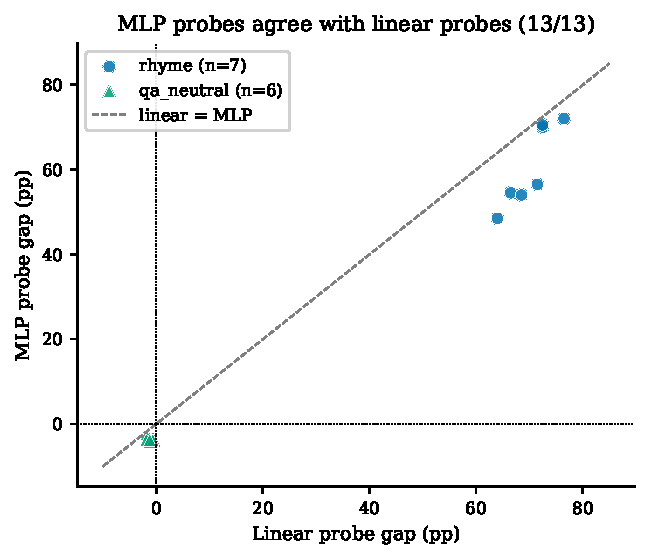
\includegraphics[width=0.85\columnwidth]{figA_mlp_agreement.pdf}
\caption{Two-layer MLP probe gap versus linear probe gap, for rhyme and
QA-neutral across six models. All 13 runs agree in sign and regime; points lie
near the diagonal for rhyme and near the origin for QA-neutral.}
\label{fig:mlp}
\end{figure}

We refit the staircase with a two-layer MLP probe (one hidden layer, ReLU)
under the same cross-validation protocol. Across six models spanning four
families (Gemma-2-2B/9B, Qwen3-1.7B/8B, Mistral-7B, Llama-3.1-8B), all 13 runs
agree with the linear probe: rhyme gaps remain large and positive
($+48$ to $+72$pp) and QA-neutral gaps remain near zero ($-2$ to $-4$pp). The
discrimination between tasks is therefore not an artifact of linear probe
capacity.

\section{Size invariance}
\label{app:size}

\begin{figure}[h]
\centering
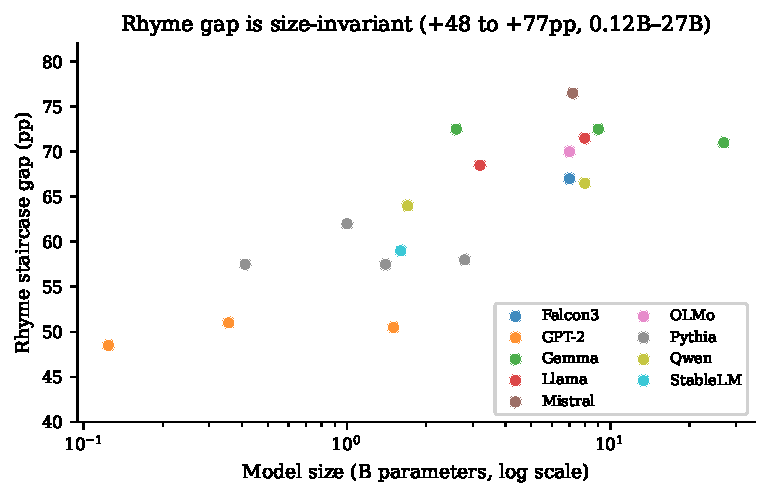
\includegraphics[width=\columnwidth]{figB_size_invariance.pdf}
\caption{Rhyme staircase gap versus model size (log scale), colored by family.
The gap is $+48$ to $+77$pp across 0.12B--27B parameters with no systematic
size trend.}
\label{fig:size}
\end{figure}

The rhyme gap is essentially flat in model size across nine families
(Figure~\ref{fig:size}), ranging from $+48.5$pp (GPT-2 small, 124M) to
$+76.5$pp (Mistral-7B) with no monotonic trend. The signal is a property of the
task and the representation, not of scale.

\section{Per-task cross-model summary}
\label{app:summary}

\begin{table}[h]
\centering\small
\begin{tabular}{@{}lcccc@{}}
\toprule
\textbf{Task} & \textbf{$n$} & \textbf{Mean} & \textbf{Median} & \textbf{Range} \\
\midrule
Rhyme & 19 & $+63.6$ & $+65.2$ & $[+48.5,+76.5]$ \\
QA-suggestive & \phantom{0}4 & $+12.7$ & $+12.4$ & $[+11.0,+14.5]$ \\
Code & 18 & $+12.0$ & $+12.0$ & $[+8.9,+15.0]$ \\
QA-neutral & 12 & $-1.2$ & $-1.2$ & $[-1.9,-0.6]$ \\
Trivia & \phantom{0}5 & $+0.0$ & $+0.0$ & $[+0.0,+0.0]$ \\
\bottomrule
\end{tabular}
\caption{Headline staircase gap (pp) per task across all evaluated models.}
\label{tab:summary}
\end{table}

Table~\ref{tab:summary} summarizes the headline gap across all models for each
task. The complete set of 116 probing experiments, including all per-layer
accuracies, bootstrap intervals, ablations, and checkpoint sweeps, is released
with the code.

\end{document}
